
\cleardoublepage


\chapter{Northeast Beam Port Modeling}

% ------------------------------------------------------------------------------
\section{Introduction}

% I'll write this last after the rest of the chapter is finished.

% ------------------------------------------------------------------------------
\section{Addition of Northeast Beam Port}


\subsection{Existing Model}

% introduce the idea of the model
% talk about the effort
In the summer of 2017, a reactor modeling effort was initiated at KSU.
% why it started
The goal of the effort was to produce, from the ground up, a python-based suite that would interpret geometric and material data related to KSU's Triga Mark II research reactor and produce input files for various transport codes.
% what has been produced so far
The model, though still currently under development, contains a majority of the features from the actual reactor, including any of those which would have a major neutronic impact.
There are 85 fuel elements, containing fresh fuel, that are able to be automatically discretized axially, radially, and azimuthally into up to 10,000 cells.
The four control rods are also included, and a user may specify their exact position to match that of in-core experiments.
The central thimble, grid plates, and source location are all also included in the core model, which is surrounded by a graphite reflector.
This model can be seen in \FIG{fig:existing}.

% the existing reactor model
\begin{figure}
\centering
\subfloat[$yz$]{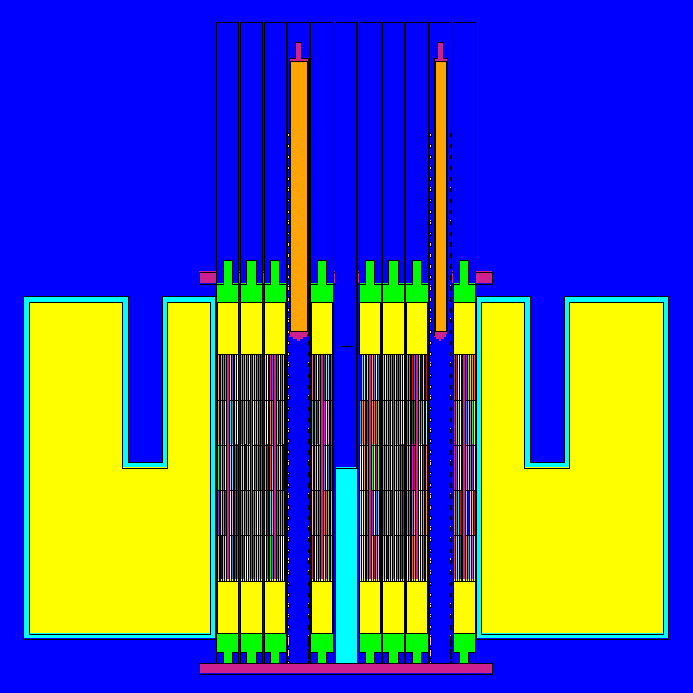
\includegraphics[height=3in]{tex/figures/existingyz.png}} 
\subfloat[$xy$]{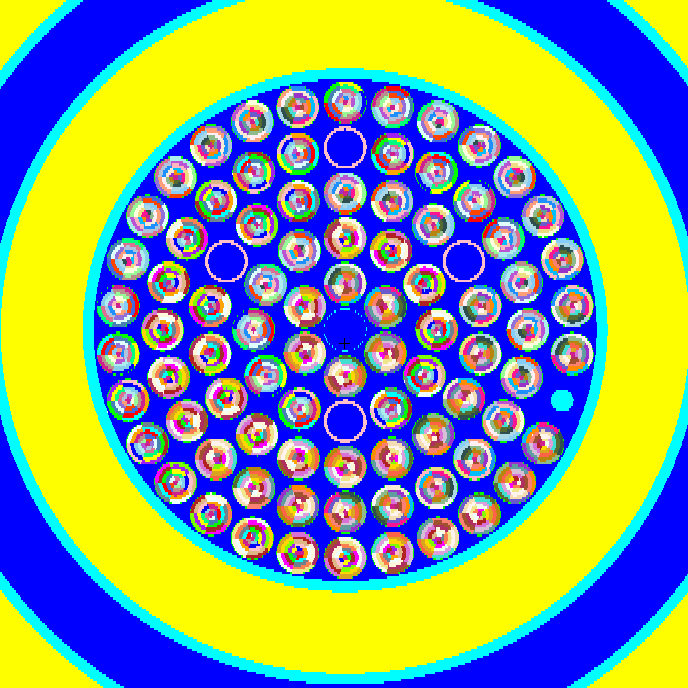
\includegraphics[height=3in]{tex/figures/existingxy.png}}
\caption[Old Reactor Model]{A $yz$ and $xy$ slice of the existing reactor model before the addition of the beam port.}
\label{fig:existing}
\end{figure}


\subsection{The Beam Port Geometry}

% introduce
Using this model as a starting point, the northeast beam port (NEBP) was then added.
% what is the beam port
The NEBP, also known as the penetrating beam port or the fast beam port, is in essence, a large collimating cavity in the reactor's structure that allows neutrons to stream from the core to the outside of the reactor.
% purpose
The primary purpose of this is to provide a monodirectional neutron source, the strength of which can be scaled easily via reactor control.
This can be used for detector calibrations and testing, neutron imaging, or sample irradiation for neutron activation analysis.
The NEBP is unique in the fact that it penetrates the graphite reflector providing, in theory, the hardest neutron spectrum of the four beam ports at KSU.
This is due to the absence of significant moderating material between the fuel and the beam port, as all other beam ports are located outside of the graphite reflector.

% isometric view of the solidworks model of the beam port
\begin{figure}[htb]
\centering
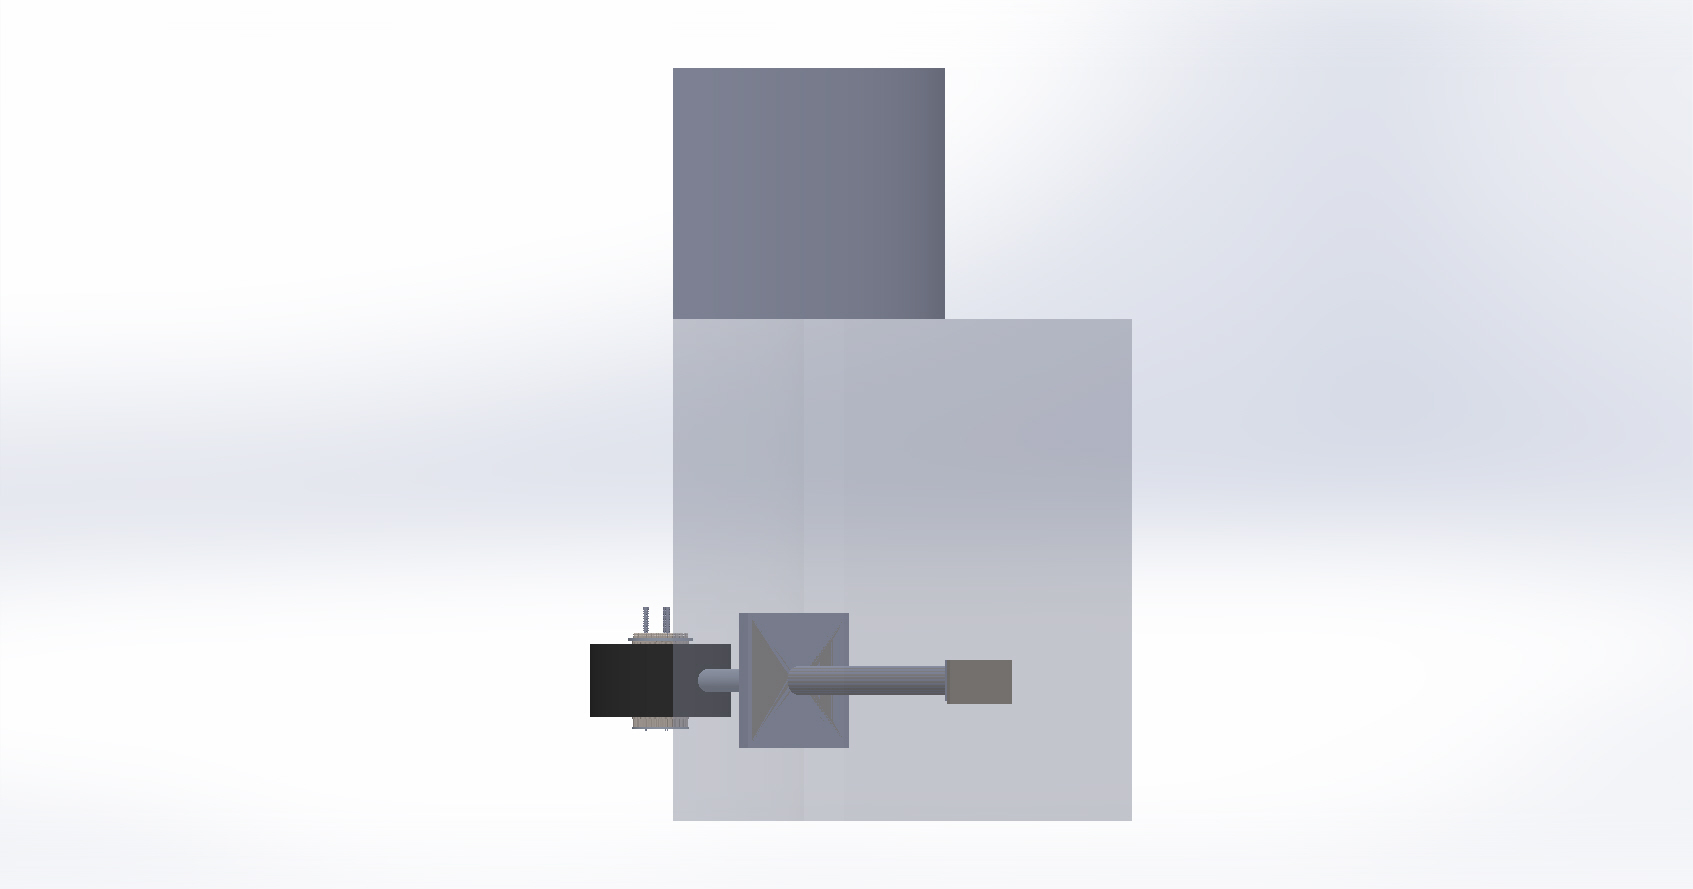
\includegraphics[height=3in]{tex/figures/solidworksangled.jpg}
\caption[Solidworks Angled NEBP]{An angled view of the NEBP with the reactor with a quarter section of the reactor structure.}
\label{fig:solidworksangled}
\end{figure}


The NEBP geometry is relatively simple.
% two sections 6 and 8 inch
It is comprised of two, six-foot, cylindrical segments; the inner and outer segments being 6" and 8" in diameter, respectively.
% coupled by shadow shield
A lead ``shadow shield" sits at the junction of these two sections to help reduce the gamma component of the outgoing particle stream.
The shadow shield is 4'x4' and 4" thick and contains a hole through the center, through which the outer portion of the NEBP's 6" section extends.
% material
The walls of each section are made of 11/32" thick aluminum.
% wooden plugs but now empty
Originally, these sections contained removable wooden plugs that would dissallow neutron to stream through; however, water leaks in the port caused damage to these plugs and at present they have been removed.

% collimator
A collimator is situated within the 8" section.
% who made it
This was designed by a KSU senior design team attempting to further constrain the neutron beam.
% describe design
The collimator is an aluminum tube of 0.75" ID and 1" OD.
An aluminum plate is affixed to this tube on the reactor side and contains a throughhole to maintain line of sight with the reactor core.
Borated polyethylene disks have been stacked around the tube to act as the primary absorption medium for collimating neutrons.
The borated polyethylene extends the entire distance of the collimator. 


\subsection{MCNP Implementation}

% mcnp with beamport geometry (zx)
\begin{figure}[htb]
\centering
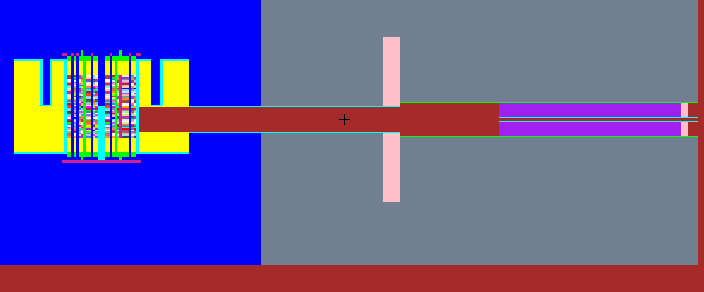
\includegraphics[height=2.5in]{tex/figures/mcnp_newxz.png}
\caption[MCNP NEBP $XZ$]{An $xz$ view of the NEBP in mcnp.}
\label{fig:mcnp_newxz}
\end{figure}

% the xy view of the nebp in mcnp
\begin{figure}[htb]
\centering
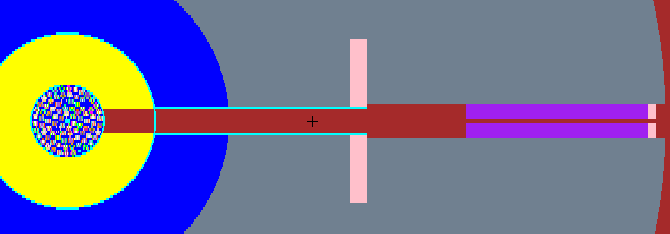
\includegraphics[height=2.1in]{tex/figures/mcnp_newxy.png}
\caption[MCNP NEBP $XY$]{An $xy$ view of the NEBP in mcnp.}
\label{fig:mcnp_newxy}
\end{figure}


% Write about the actual implementation
The NEBP itself consists primarily of cylinders and planes, so its implementation in the model was relatively straightforward.
The surrounding concrete structural region was modeled as a large cylindrical cell, with the assumption that the geometric intracies a great distance from the NEBP would have a minimal effect on the flux in the NEBP.
As described above, the NEBP, including both sections and the shadow shield, was added within this concrete region.
% hole in the graphite reflector
A penetration was added to the existing graphite reflector.
The reactor documentation was unclear about some specifics regarding this penetration, so it was assumed that it was not radially encased by any aluminum, but the aluminum surrounding the reflector was left intact to not let water in.
The materials used for the NEBP can be seen in \TAB{tab:nebp_materials}.
Material data in the model came from {\tt pyne}.


% table that contains the material data for the model
% density of steel 8.03

\begin{table}[h]\centering
\label{tab:nebp_materials}
\caption{Materials used in the NEBP model.}
\begin{tabular}{ r c l }
\toprule
\textbf{Material} & \textbf{Density} $g/cm^3$ & \textbf{Composition (Wgt. Fraction)} \\
\midrule
Aluminum & 2.7 & $^{27}$Al (1.000) \\
\midrule
Lead & 11.34 & $^{204}$Pb (0.0138)  $^{206}$Pb (0.2396) \\
        & & $^{207}$Pb (0.2207)  $^{208}$Pb (0.5259) \\
\midrule
Air & 0.001239 & $^{12}$C (0.0001)  $^{14}$N (0.7147) \\
        & & $^{16}$O (0.205)  $^{40}$Ar (0.0346) \\
\midrule
Borated Polyethylene & 0.95 & $^{1}$H (0.1253)  $^{2}$H (0.000028) \\
                       &  & $^{10}$B (0.0184)   $^{11}$B (0.0816) \\
                       &  & $^{12}$C (0.7657)   $^{13}$C (0.0090) \\
\midrule
Concrete & 2.4 &  $^{1}$H (0.0221) $^{2}$H (0.00000509) \\
& &         $^{12}$C (0.002458)  $^{13}$C (0.0000288) \\
& &           $^{16}$O (0.5741)  $^{17}$O (0.000232) \\
& &          $^{23}$Na (0.0152)   $^{24}$Mg (0.000988) \\
& &          $^{25}$Mg (0.00013)   $^{26}$Mg (0.000149) \\
& &          $^{27}$Al (0.01998)   $^{28}$Si (0.2802) \\
& &          $^{29}$Si (0.0147)  $^{30}$Si (0.010066) \\
& &          $^{39}$K (0.0093)   $^{40}$K (0.0000012) \\
& &          $^{41}$K (0.000709)  $^{40}$Ca (0.04157) \\
& &          $^{42}$Ca (0.00029)    $^{43}$Ca (0.00006223) \\
& &          $^{44}$Ca (0.00098)   $^{46}$Ca (0.00000197) \\
& &          $^{48}$Ca (0.00009622)    $^{54}$Fe (0.00036) \\
& &          $^{56}$Fe (0.00592)   $^{57}$Fe (0.000139) \\
& &          $^{58}$Fe (0.0000189) \\
\midrule
Steel & 8.03 & $^{12}$C (0.00039536233)  $^{13}$C (0.0000046336713) \\
& &            $^{28}$Si (0.0045932784) $^{29}$Si  (0.00024167903) \\
& &            $^{30}$Si  (0.00016499257) $^{31}$P  (0.0002299977) \\
& &            $^{32}$S  (0.00014207158)  $^{33}$S  (0.0000011567992) \\
& &            $^{34}$S  (0.0000067532956) $^{36}$S  (0.000000016825336) \\
& &            $^{50}$Cr  (0.007929925)   $^{52}$Cr  (0.1590272) \\
& &            $^{53}$Cr  (0.018379631)   $^{54}$Cr  (0.0046613454) \\
& &            $^{55}$Mn  (0.0099999)   $^{54}$Fe  (0.03961618) \\
& &            $^{56}$Fe  (0.64489415)   $^{57}$Fe  (0.015159803) \\
& &            $^{58}$Fe  (0.0020528512)  $^{58}$Ni  (0.062157351) \\
& &            $^{60}$Ni  (0.024767425)  $^{61}$Ni  (0.0010945963) \\
& &            $^{62}$Ni  (0.003547273)  $^{64}$Ni  (0.00093242912) \\
\bottomrule
\end{tabular}
\end{table}

\clearpage

% ------------------------------------------------------------------------------
\section{Fission Rate Tallying and Steady-State Source Generation}
\subsection{SDEF Generation}

% the goal is transport, so no kcode
The ultimate goal here is to obtain, via simulation, the flux departing from the beam port.
However, the existing model is setup only for KCODE problems.
The difficult nature of this transport problem, due to the low probability of a simulated particle streaming down the collimator and exiting the reactor, requires some form of variance reduction.
Because of an incompatibility between KCODE problems and the code ADVANTG (selected for variance reduction and used to generate weight windows), this problem must first be converted into an SDEF-type problem.
This conversion required the collection of spatially-dependent fission site data.
This ``fission map'' could provide the set of probability vectors to inform the source sampling in the steady-state problem.
This was done in the following way.
First, the fuel cells were discretized axially and radially.
It was decided that 40 axial sections and 5 radial sections were used for each of the 85 fuel elements to create a total of 17,000 individual cells.
Then a fission rate tally was created for these cells.
This was done using an F4 tally (flux averaged over a cell) with an FM (tally multiplier) card which would multiply the flux by the total fission cross section for the fresh fuel material.
With these tallys in place, the KCODE problem was then run for a total of 4,400 cycles where the first 10 were discarded and each cycle consisted of 100,000 particles.

After running this problem, a python script was used to parse the output and generate an SDEF source to be used in the next step.
This card is shown here.

\begin{center}
{\tt SDEF ERG=D1 RAD=D2  AXS=0 0 1  POS=D3  EXT=FPOS=D4}
\end{center}

The {\tt ERG} (energy) distribution used for the source was MCNP's built-in Watt spectrum, indicated simply by a {\tt -3} on the source probability card.
The source's spatial distribution is a series of cylinders co-located with the respective fuel elements within the core.
The {\tt POS} (position) variable contained the center points of each of the fuel elements, whose probability of sampling is proportional to their integrated fission rate.
The {\tt EXT} (extent) variable means length of the cylinder, in this case the length of the fuel meat, and refers to a series of distributions dependent on the {\tt POS} of the fuel.
Because base MCNP doesn't easily allow for nested dependent distributions, the {\tt RAD} (radial) distribution was considered an independent variable, and the distribution used was the normalized, averaged radial fission rate across each fuel element.

\subsection{Fission Tally Results}
Along with the source, several plots were made of this fission rate data.

% the fission rates tallied inside a fuel element
\begin{figure}[htb]
\centering
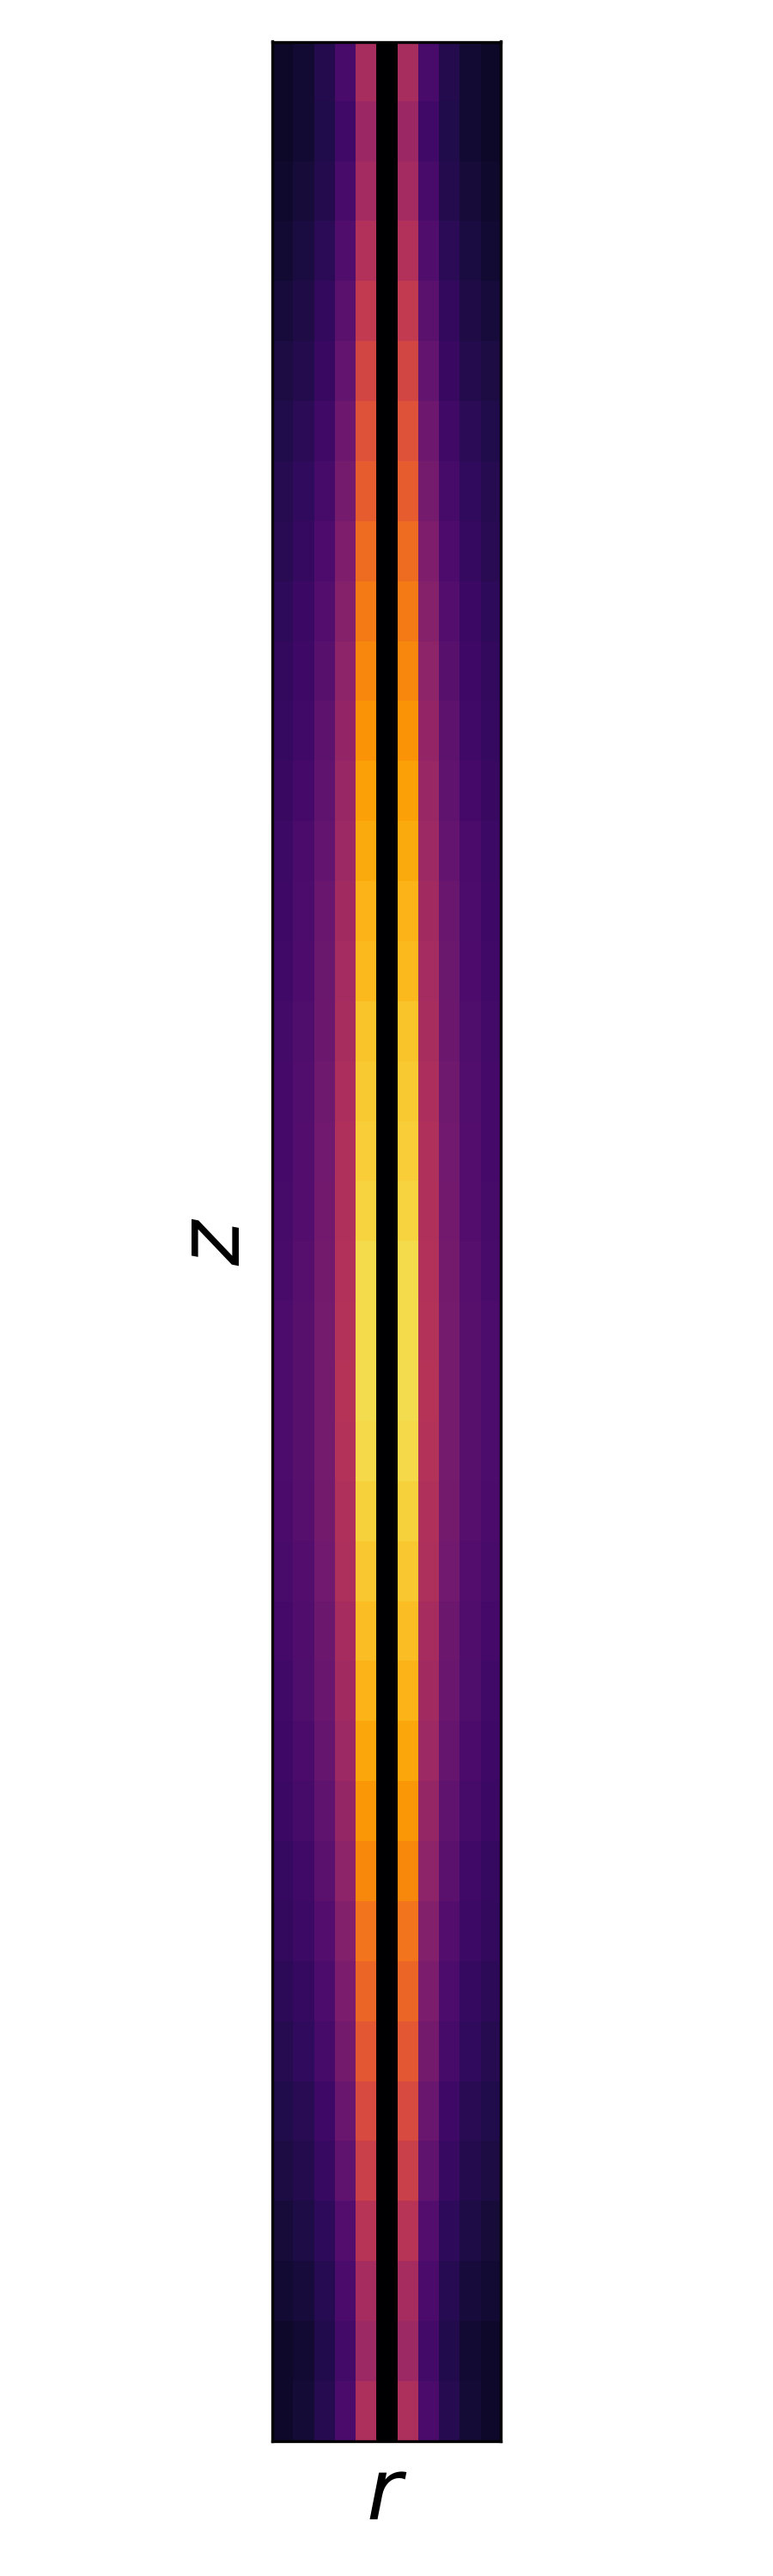
\includegraphics[height=4in]{tex/figures/rr_dist_B1.png}
\caption[Fission Rate Dist. B1]{The fission rate distribution within the element B1.}
\label{fig:rr_dist_b1}
\end{figure}

% talk about the B1 element plot
The heatmap in \FIG{fig:rr_dist_b1} demonstrates how the fissions are distributed within a typical fuel element.
Because there was no azimuthal discretization in the tallies, the values here are rotationally symmetric.
Although it is hard to draw any quantitative conclusions from this image, it is useful for visualizing fission rates within an element.
The fission rate appears to be a maximum at the center of the rod, both axially and radially.

% the radial reaction rate density within the B ring
\begin{figure}[htb]
\centering
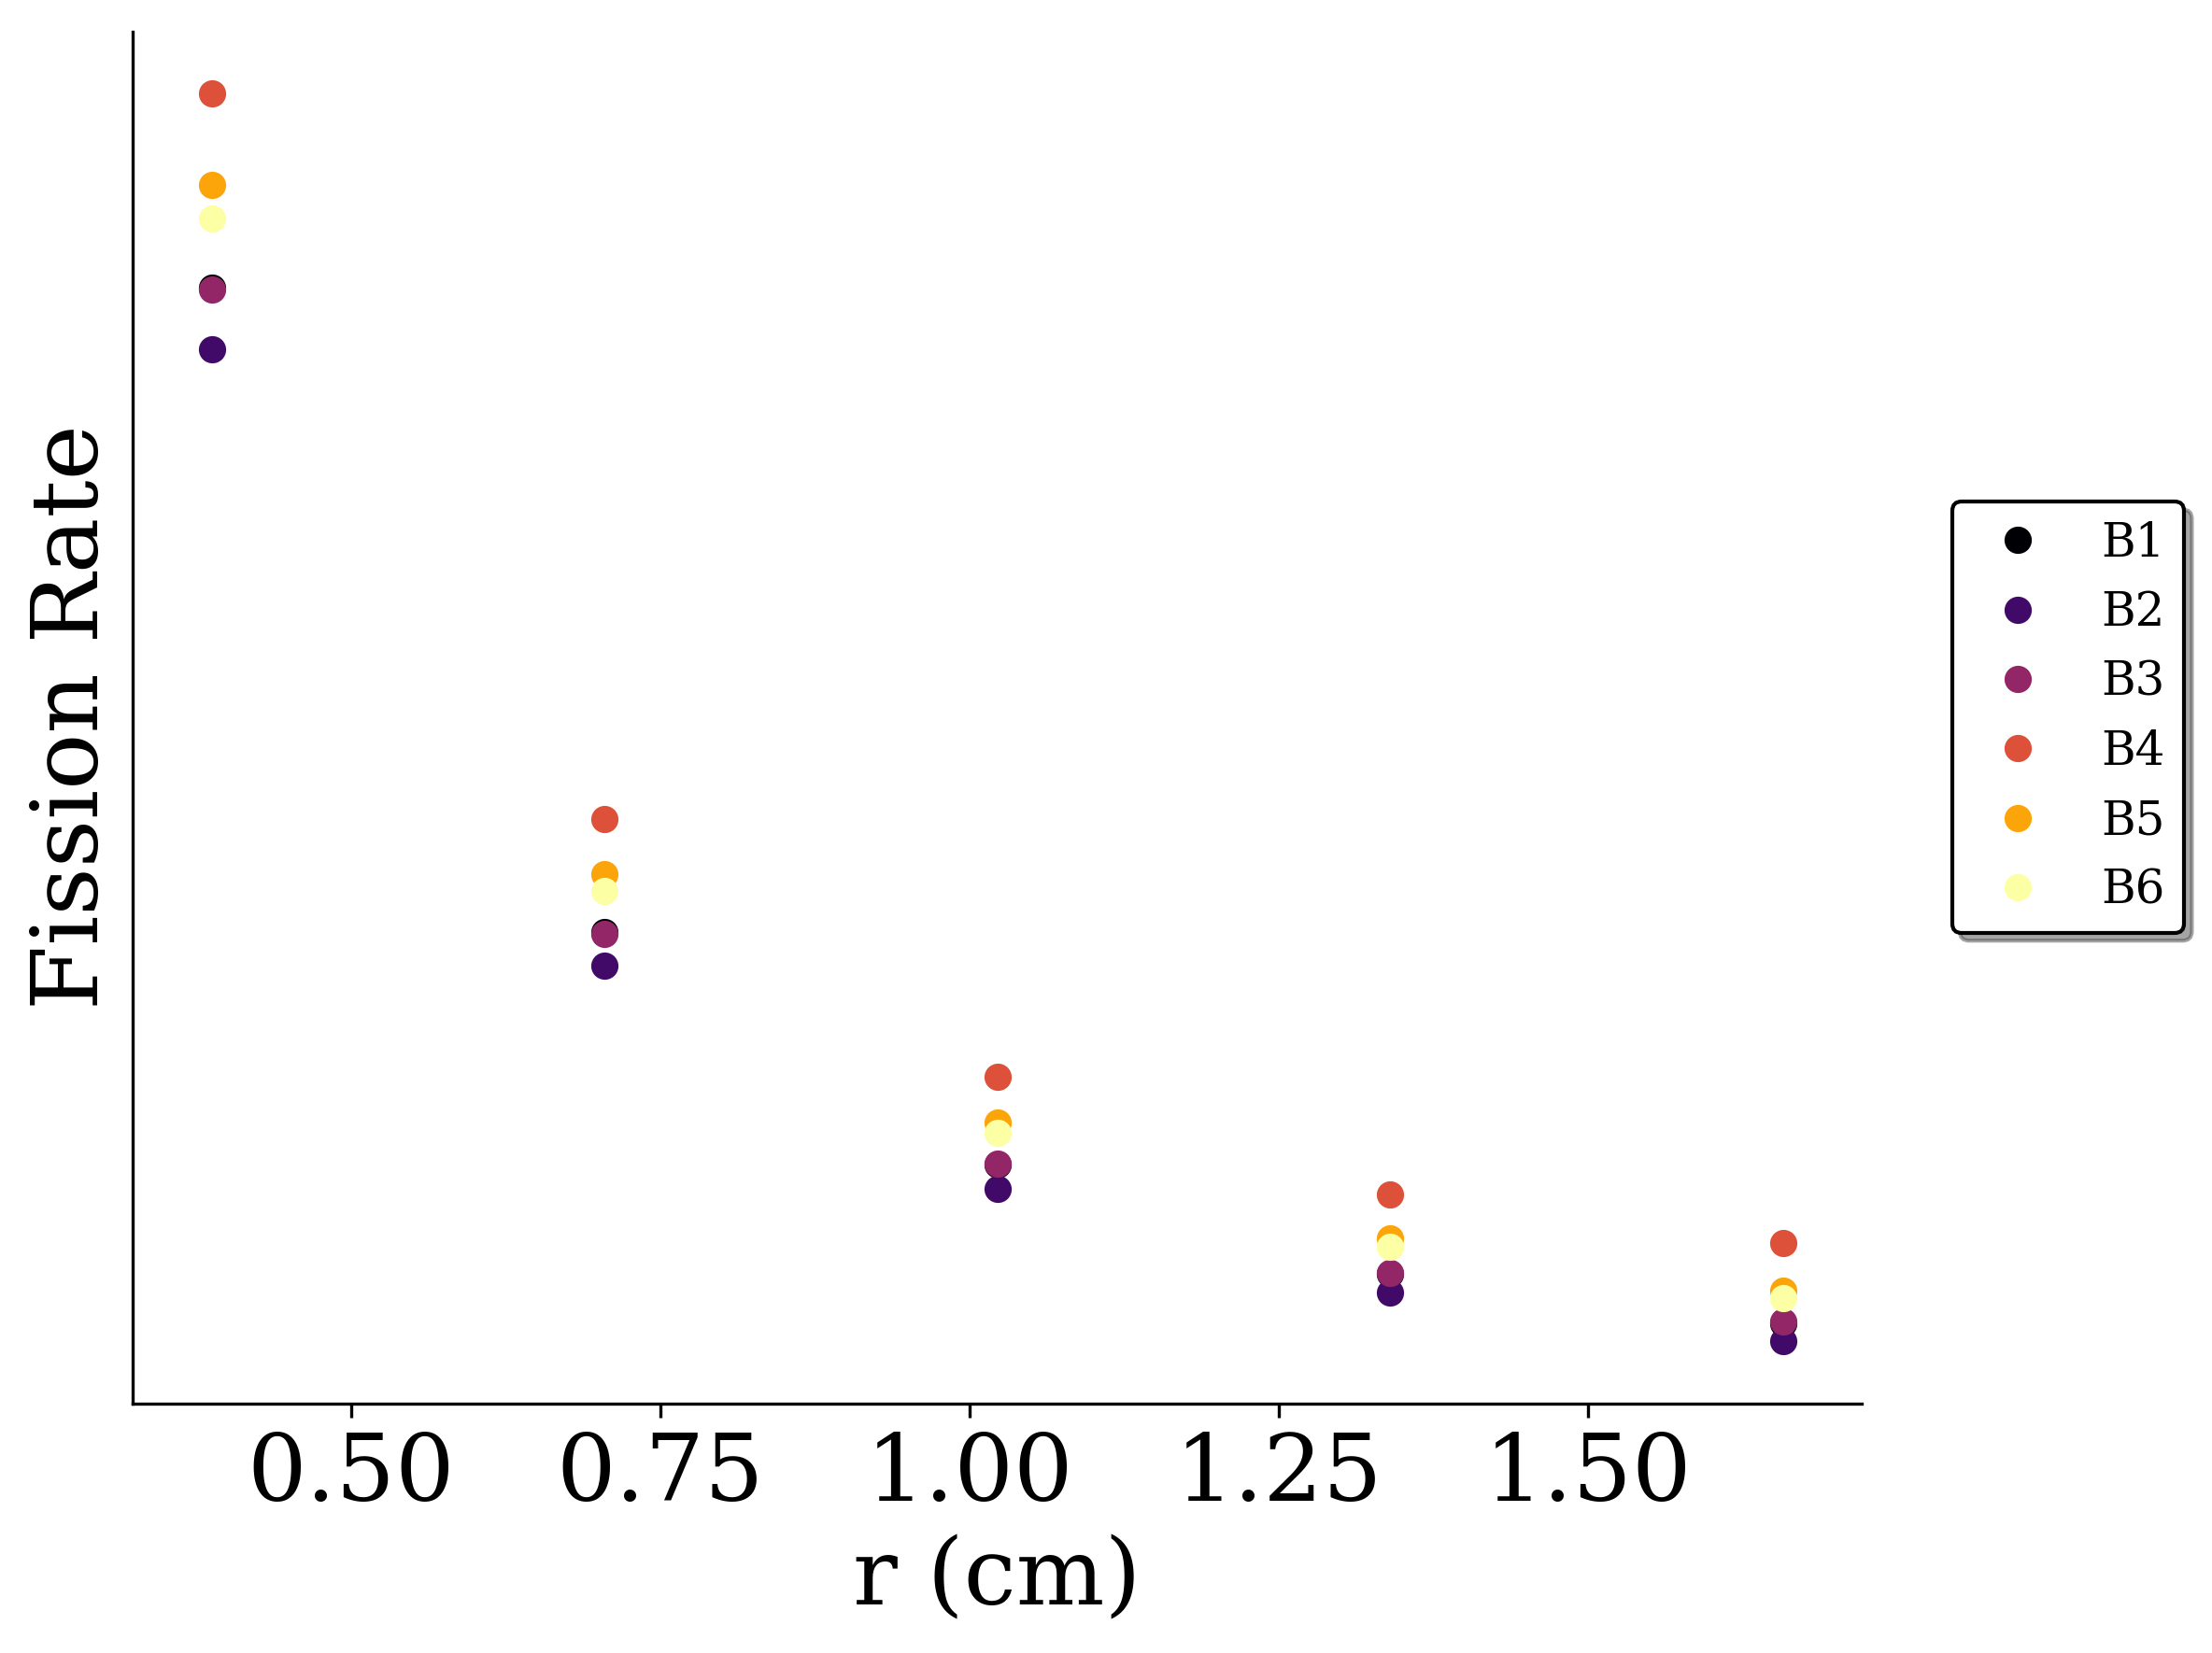
\includegraphics[height=4in]{tex/figures/radial_rr_density_B.png}
\caption[Radial Fission Rate Density B]{The radial fission rate within the B ring.}
\label{fig:radial_rr_density_B}
\end{figure}

In \FIG{fig:radial_rr_density_B}, one can see the radial behavior of the fission rates within ring B.
Although the curves here are different, they differ primarily in magnitude and not shape.
The other rings not pictured here all show similar behavior.
The fission rate density is highest towards the center of the rod and lowest in the outermost region.

% the axial reaction rate densities
\begin{figure}[htb]
\centering
\subfloat[B Ring]{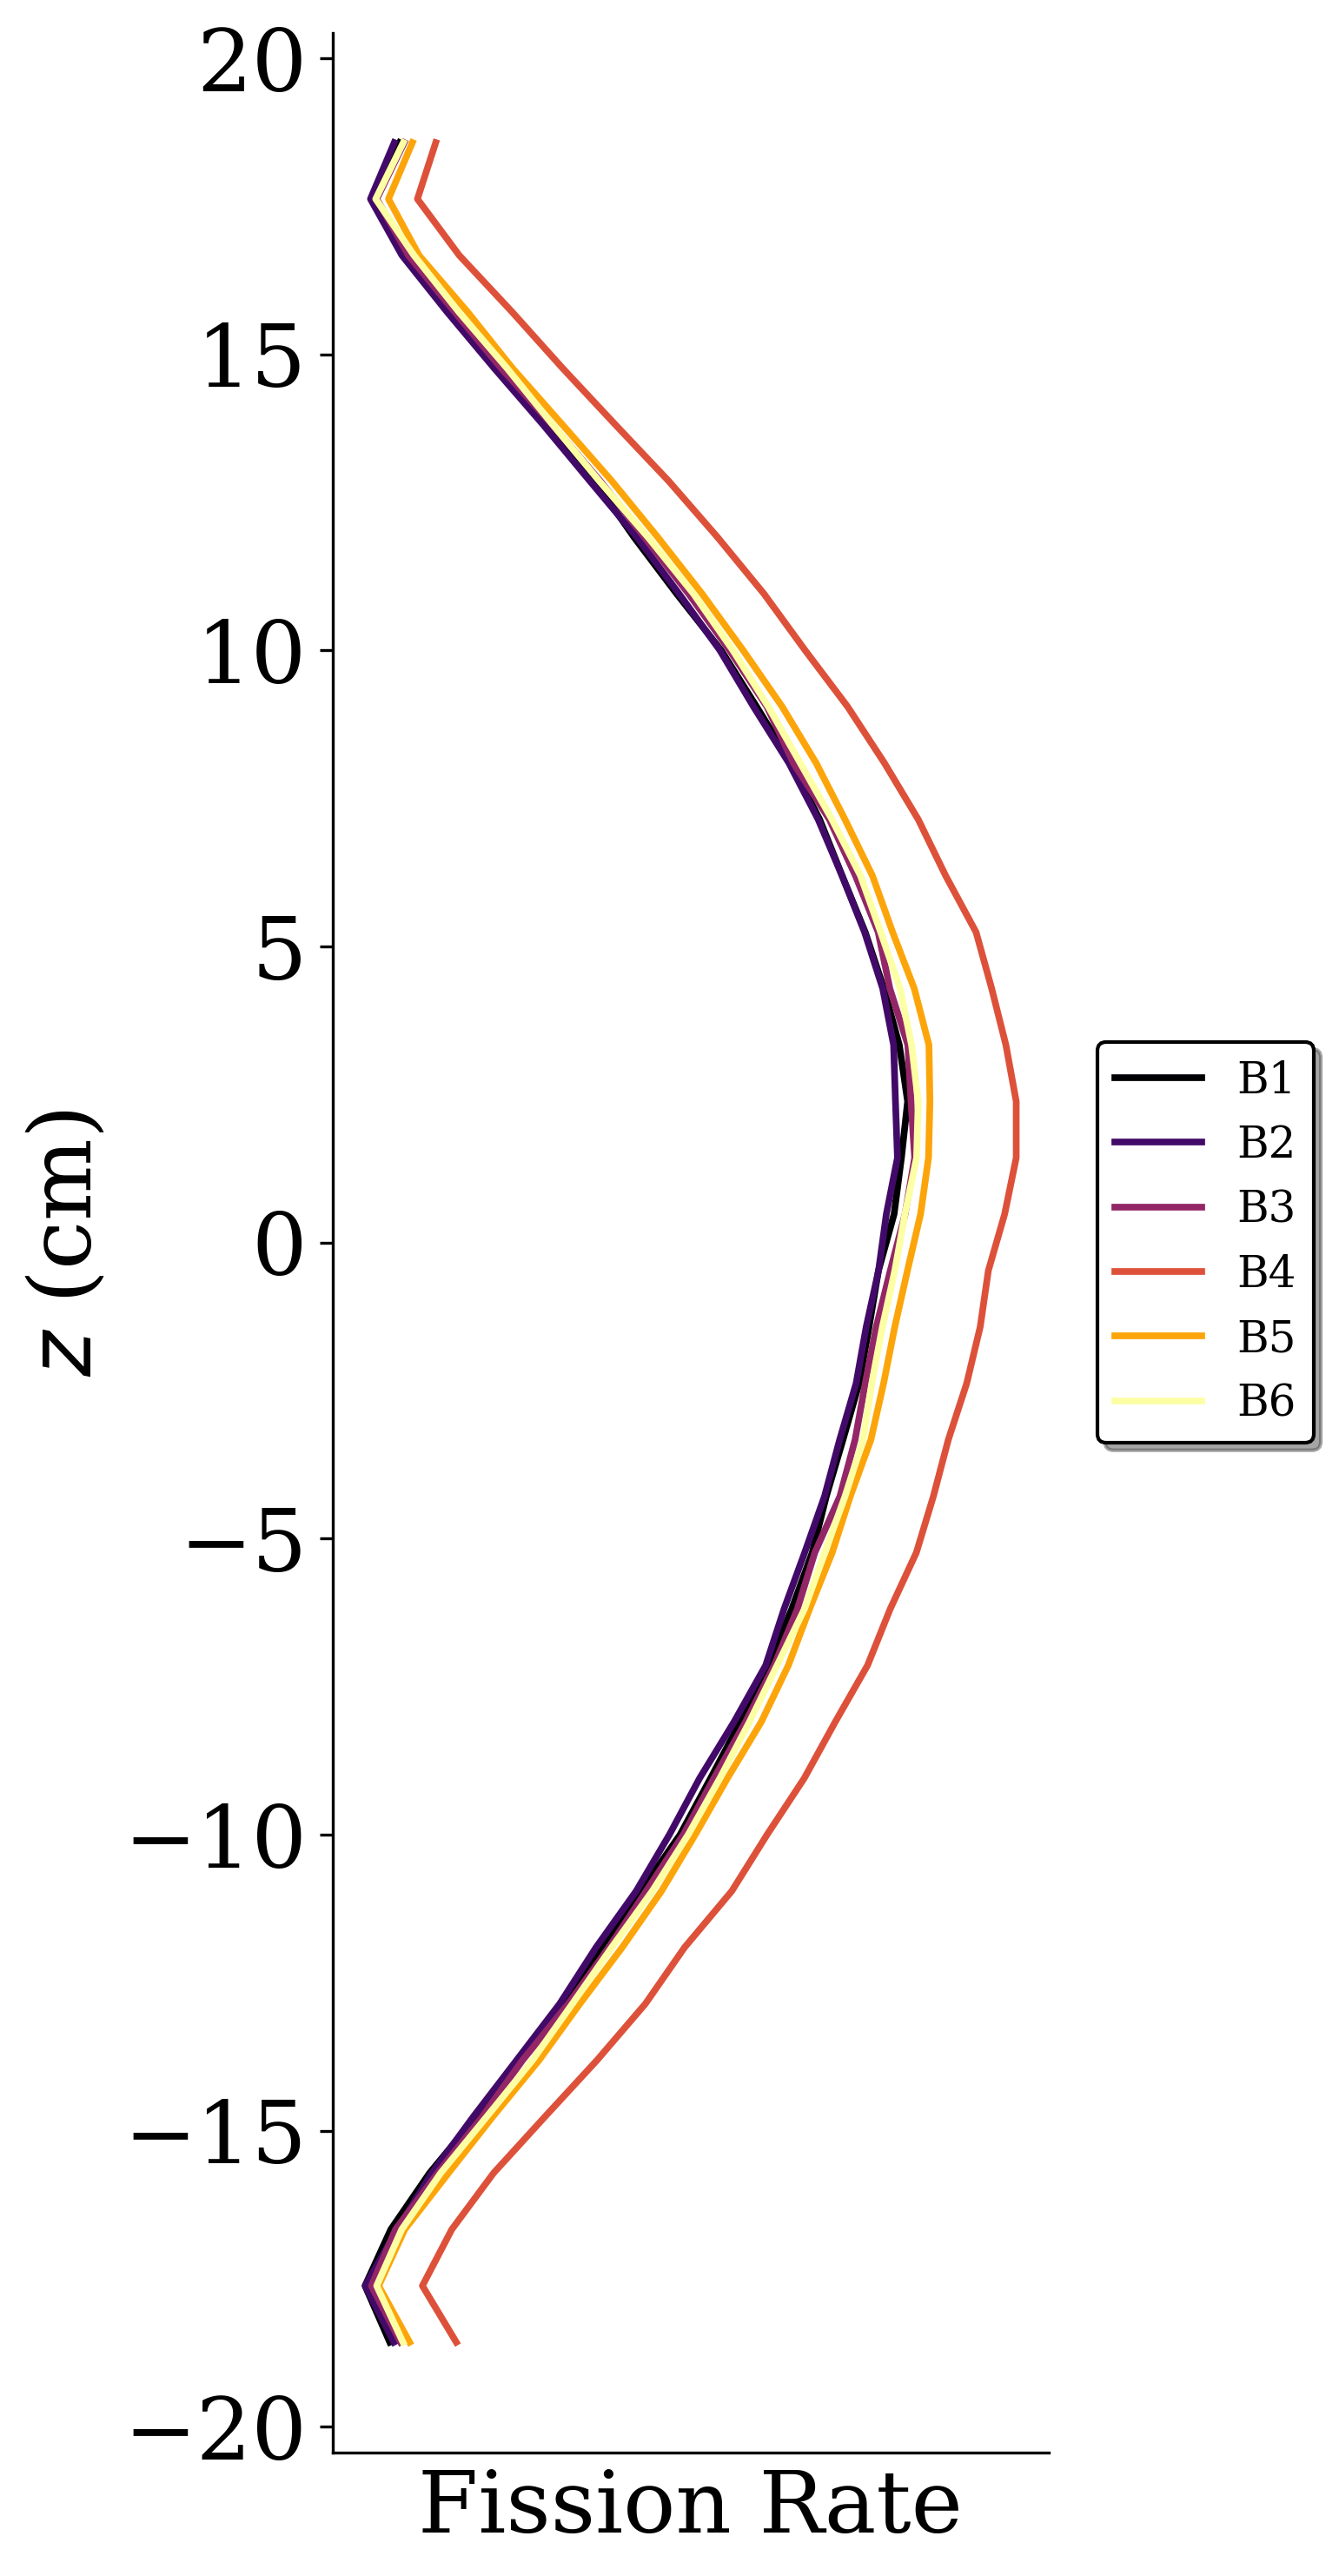
\includegraphics[height = 4in]{tex/figures/axial_rr_density_B.png}} 
\subfloat[C Ring]{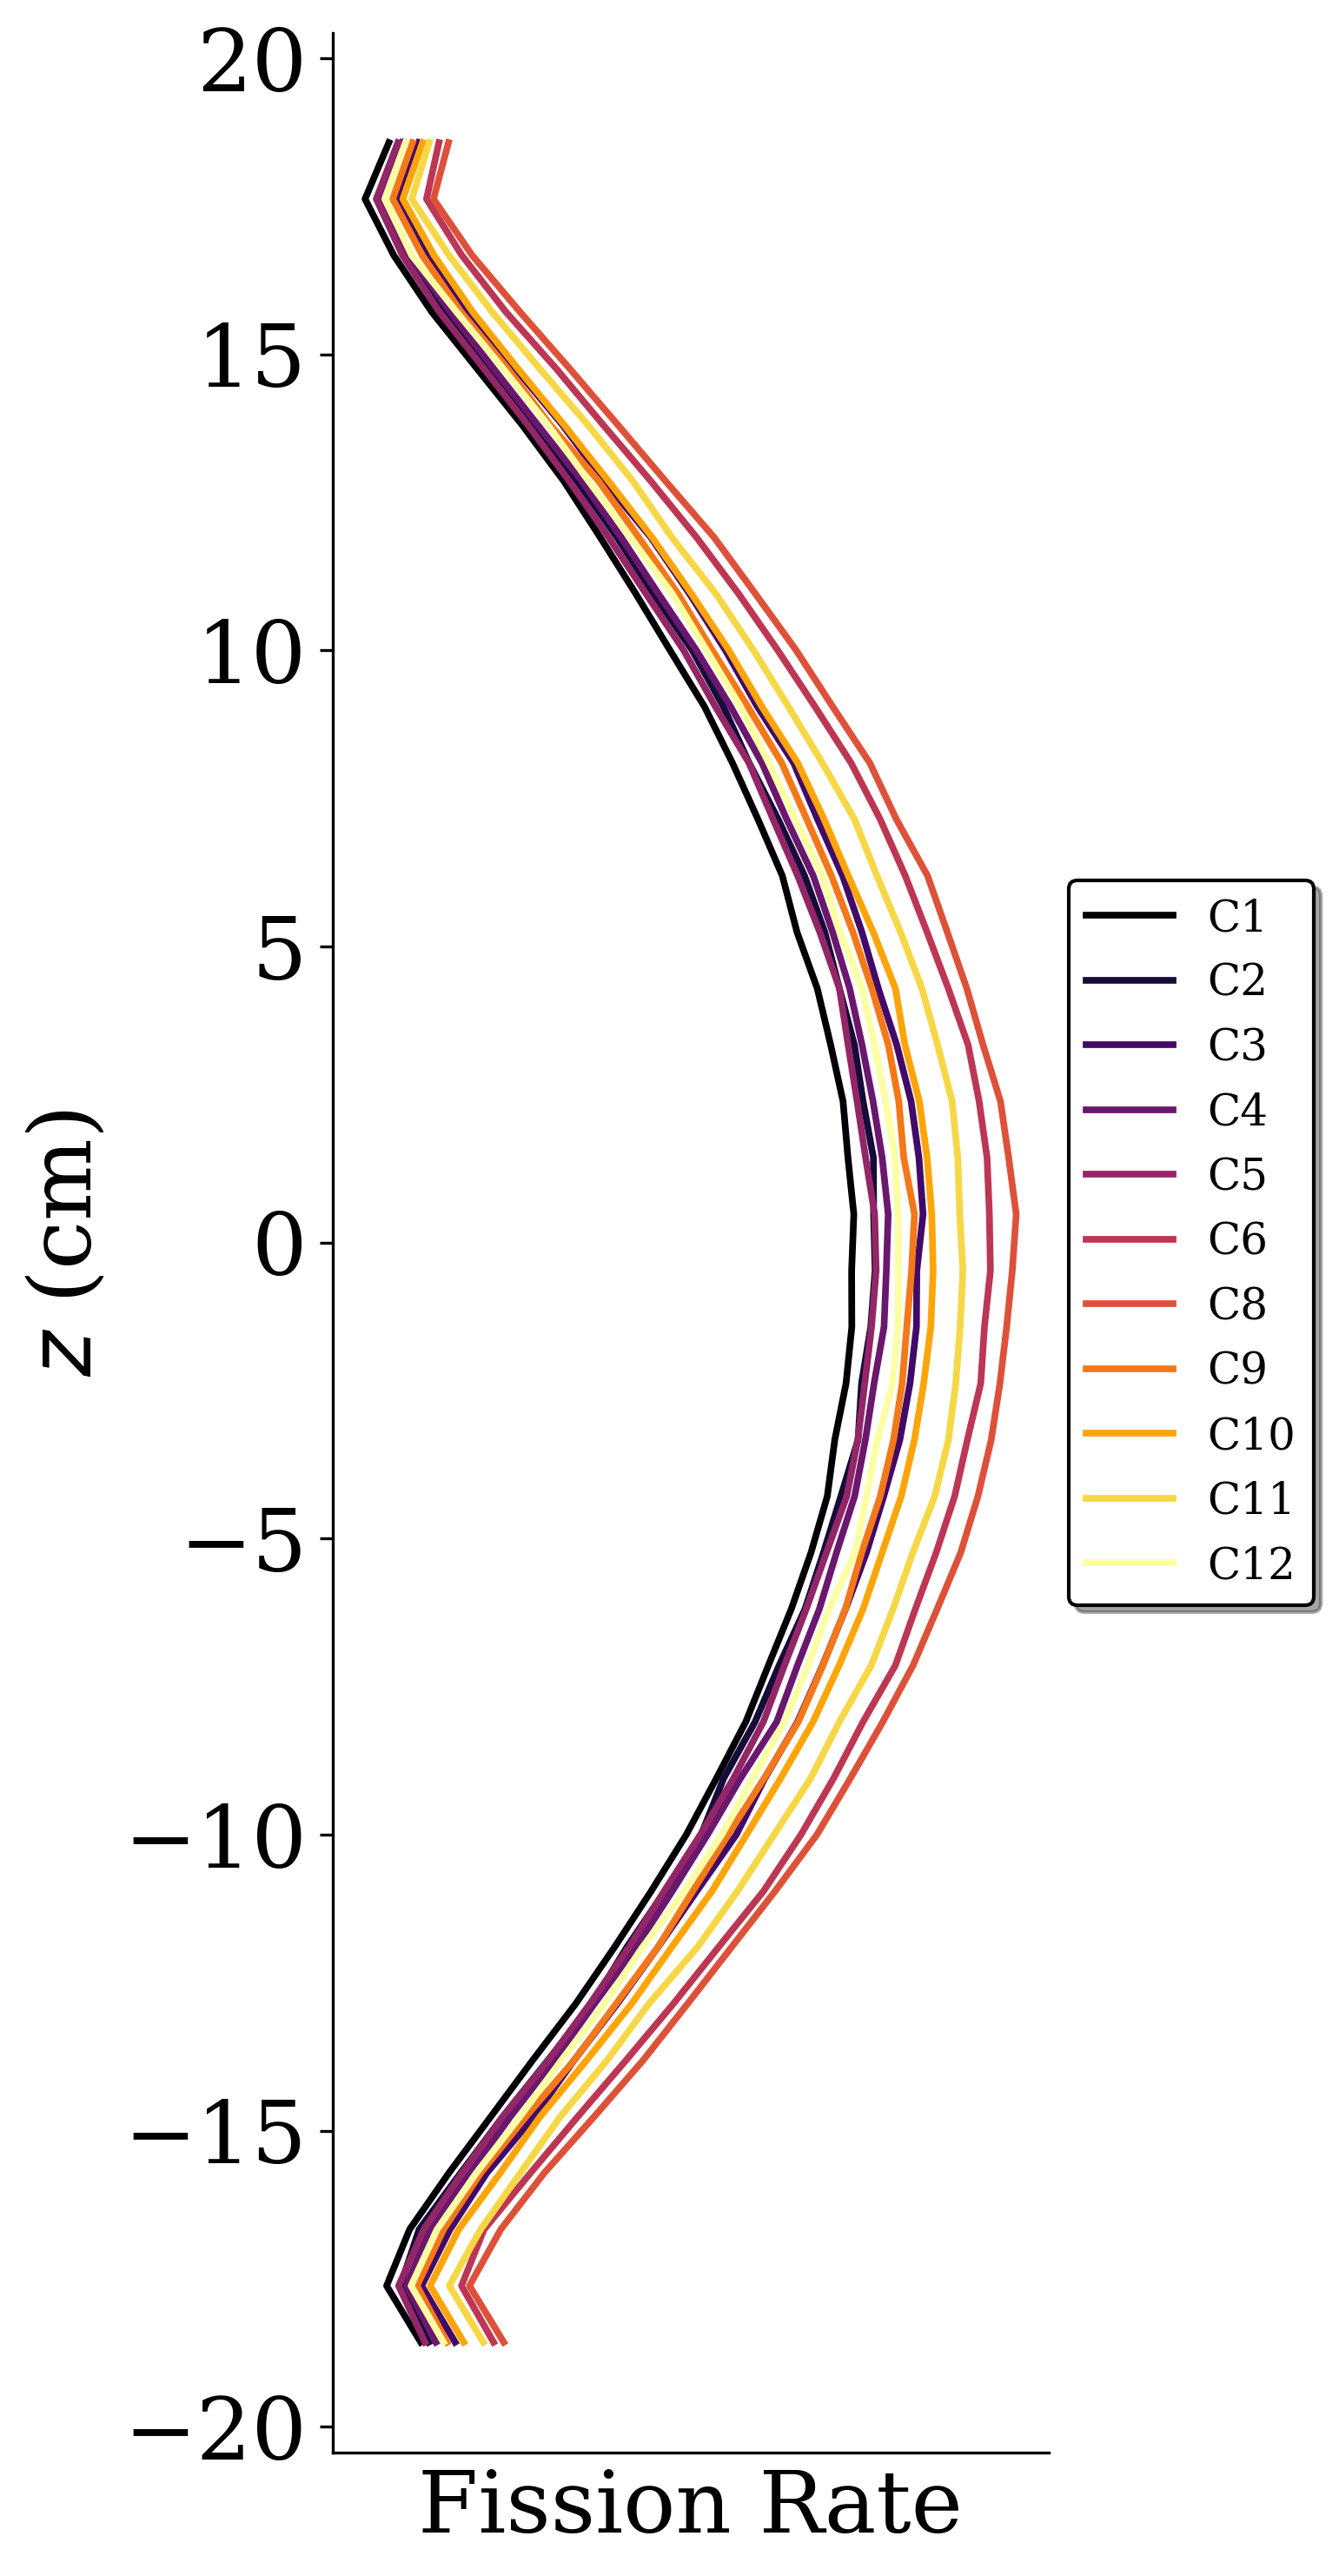
\includegraphics[height = 4in]{tex/figures/axial_rr_density_C.png}}
\subfloat[D Ring]{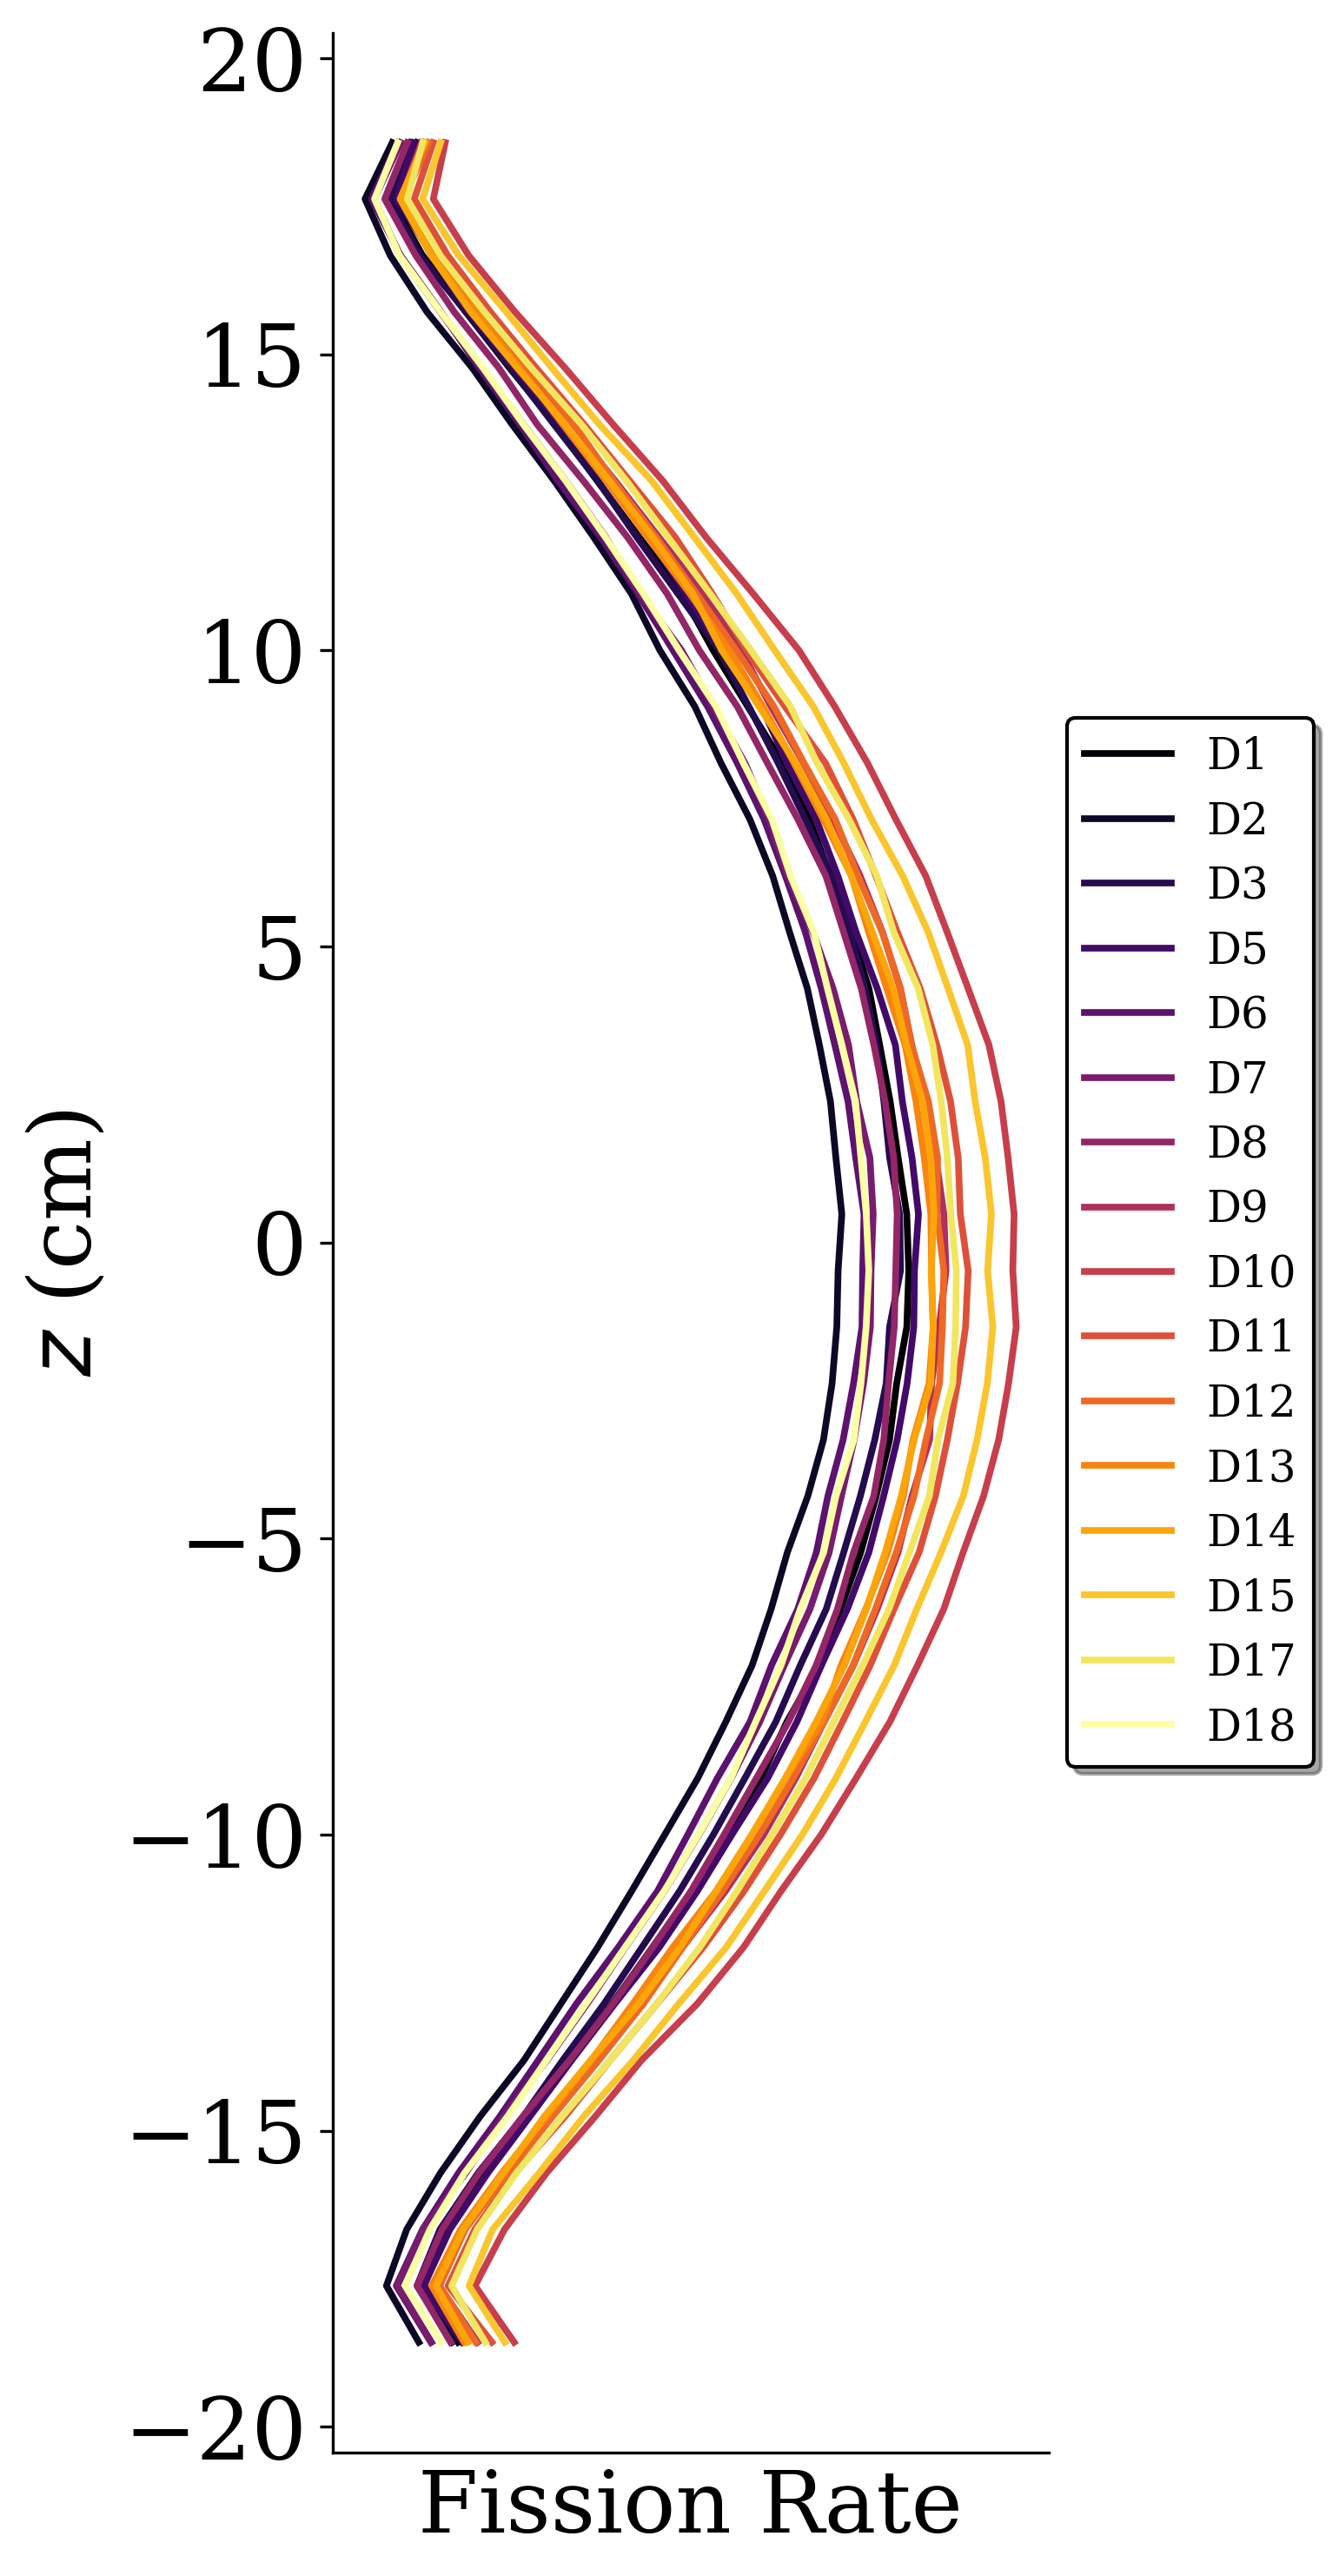
\includegraphics[height = 4in]{tex/figures/axial_rr_density_D.png}}\\
\subfloat[E Ring]{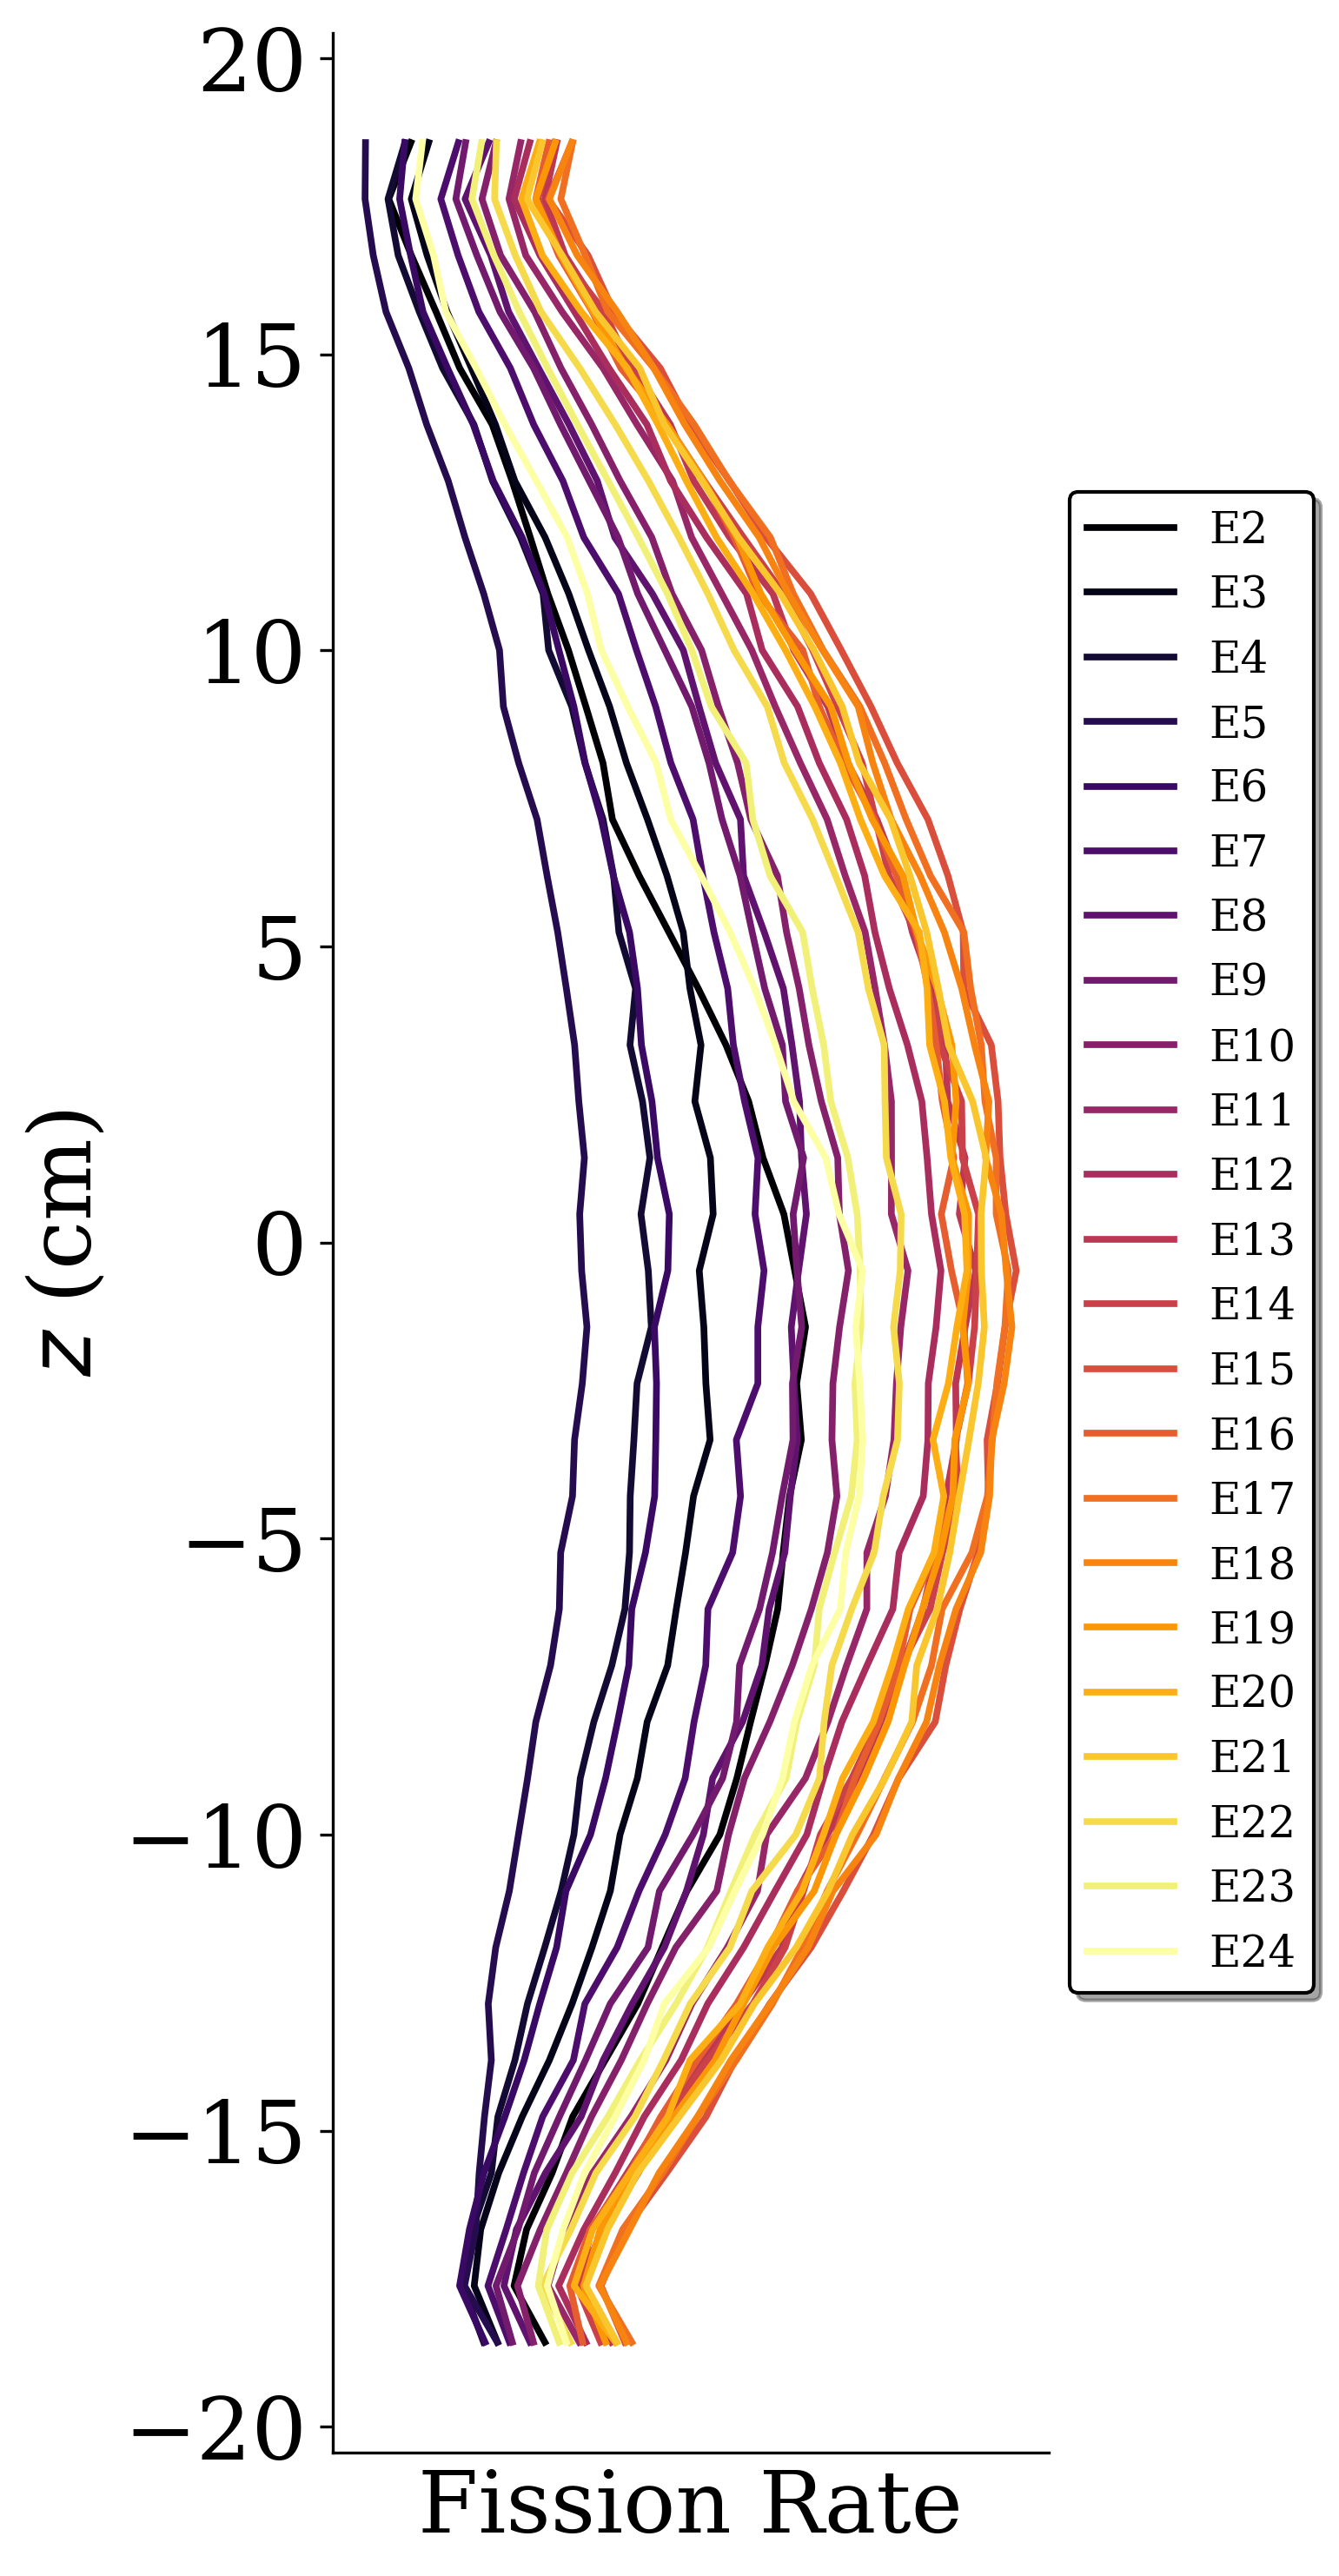
\includegraphics[height = 4in]{tex/figures/axial_rr_density_E.png}} 
\subfloat[F Ring]{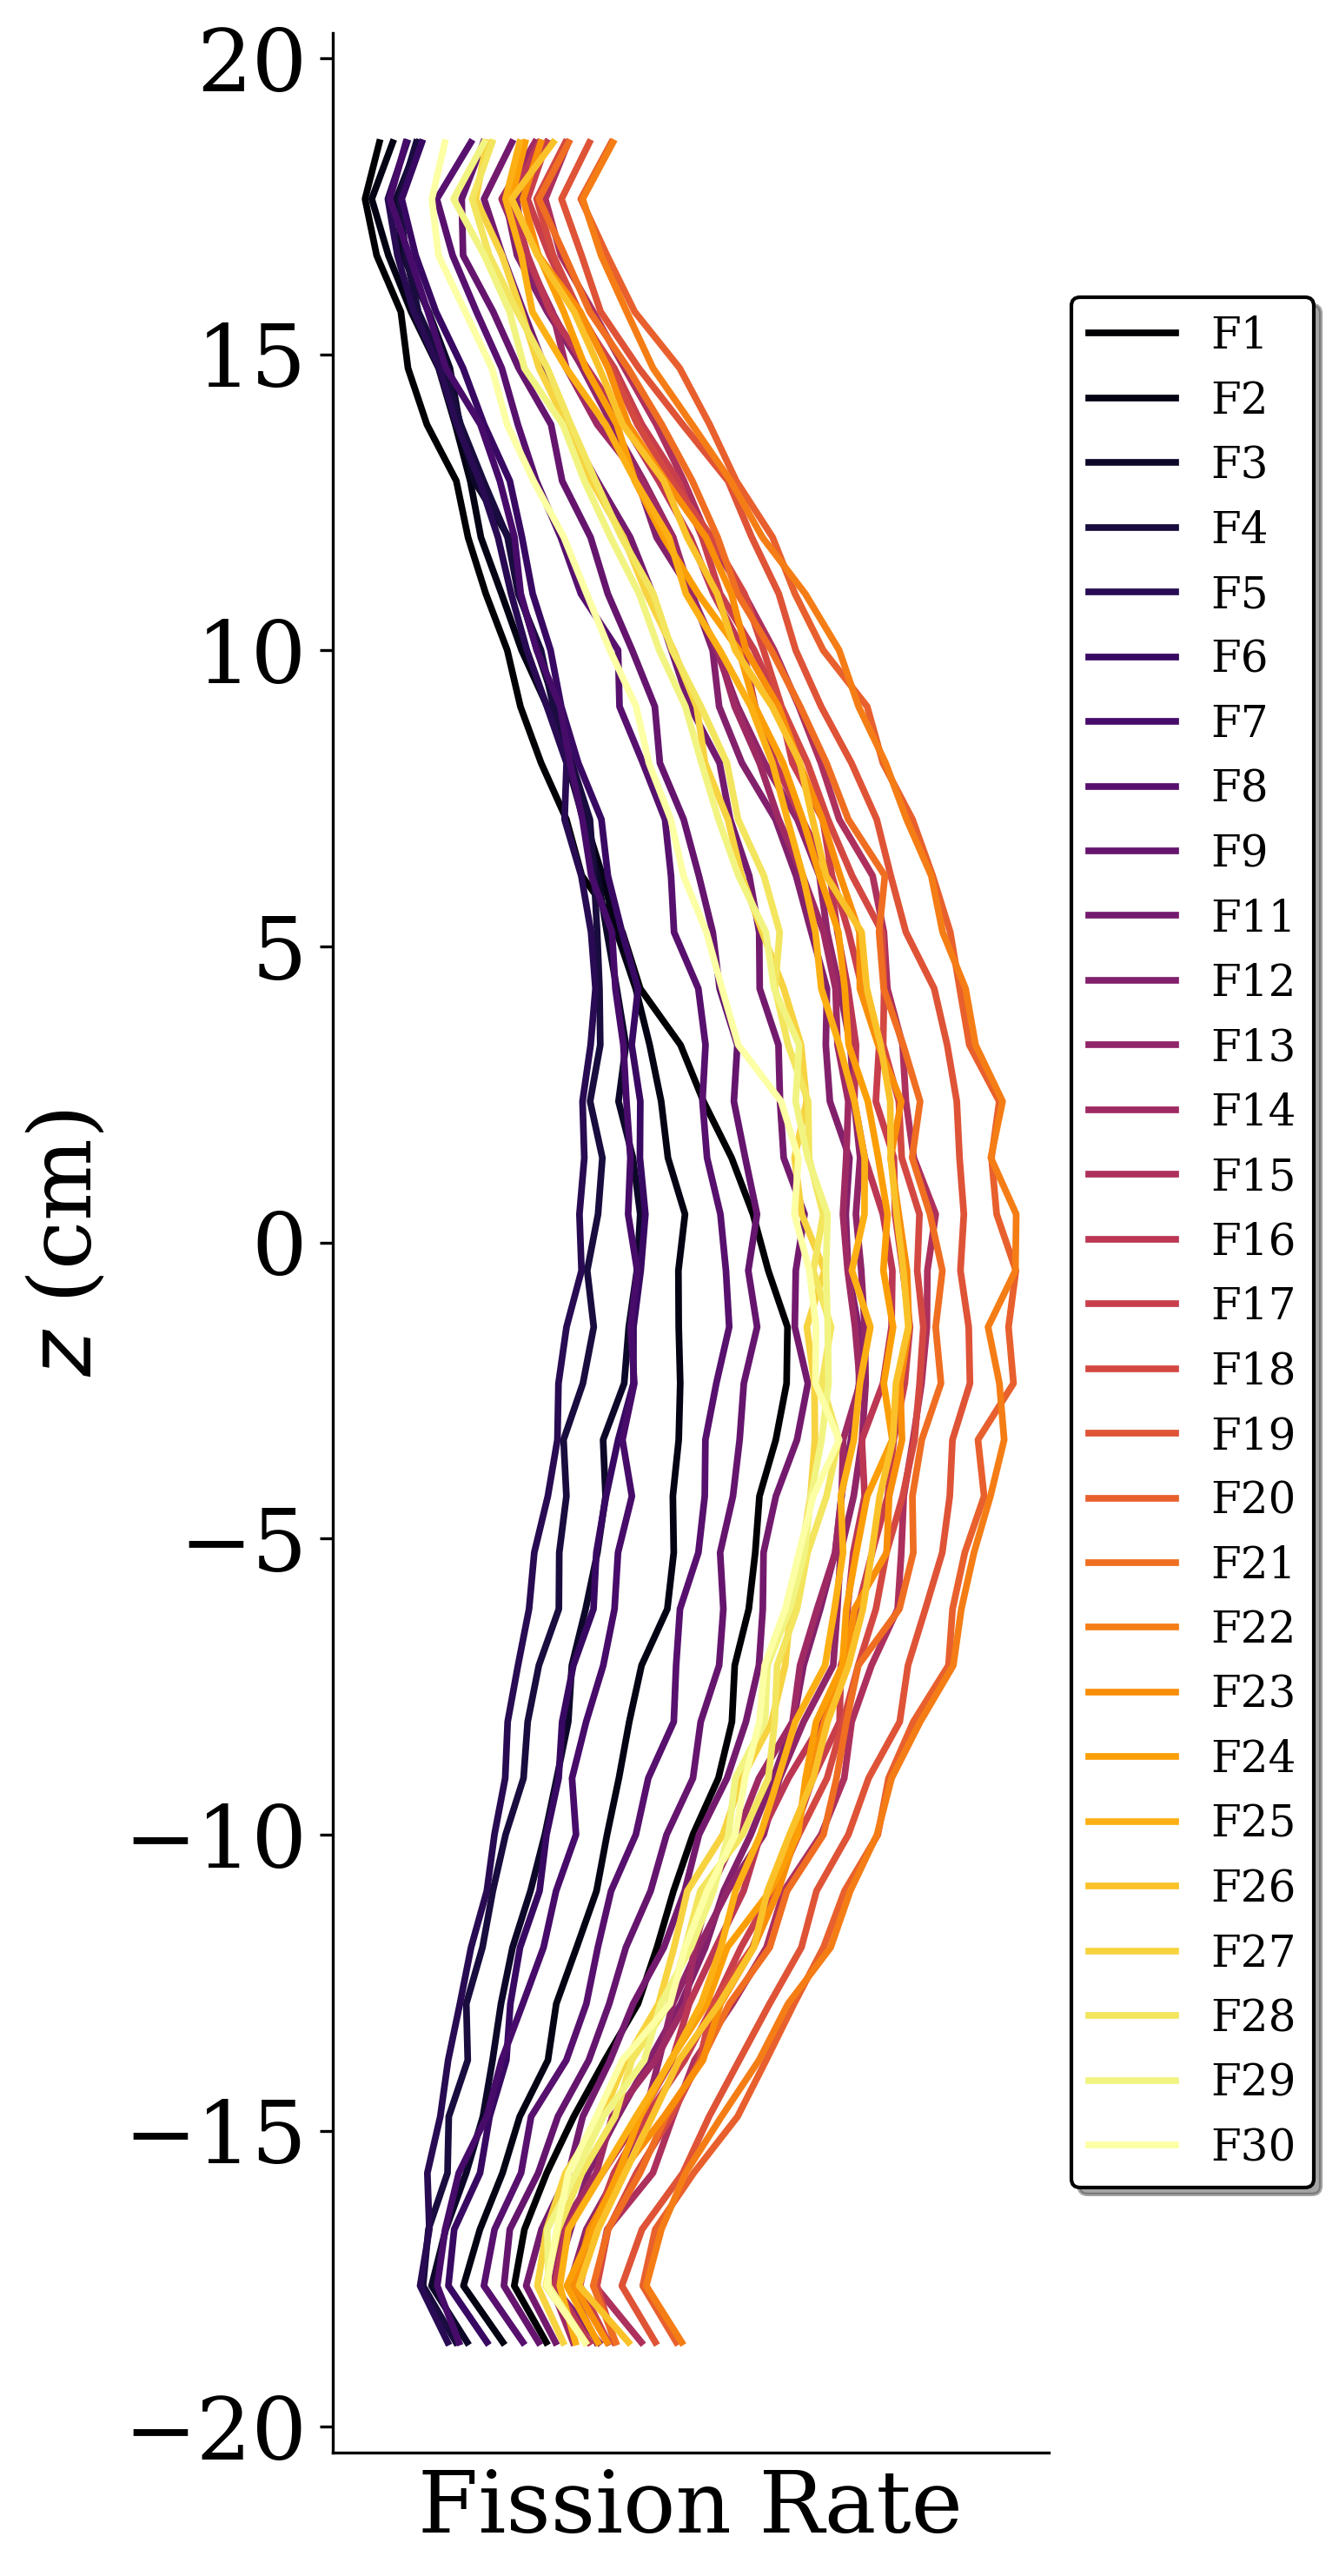
\includegraphics[height = 4in]{tex/figures/axial_rr_density_F.png}} 
\caption[Axial Fission Rates]{The axial fission rates within each ring of the core.}
\label{fig:axial_rr_density}
\end{figure}

\clearpage

\FIGURE{fig:axial_rr_density} shows the axial fission rate densities within each ring of the core.
Each of these rings shows a cosine-like distribution with a slight upturn at each extrema.
Neutron flux within a {\it roughly} cylindrical geometry, like a reactor core, will {\it roughly} exhibit a cosine shape, which causes a similar shape for the fission distribution.
The upturn is caused by the graphite on each end of the fuel elements which reflects neutrons back towards the rod.
There are two rings in particular that show additional behavior outside of these two phemonena.
The first is the depression within the B ring below 0 $cm$.
This is caused by the central thimble, which currently occupies the A1 location.
Moderating water which would normally occupy that location is replaced by this thimble which is currently modeled as an aluminum rod that extends halfway up the core.
This lack of neutron moderation means lower thermal flux in that region and results in the depression.

The second is the depressed fission rate within the lower region of F1-F9.
This is caused by the addition of the NEBP.
Recall, the beam port includes a penetration within the graphite reflector. 
This penetration is situated 8.3 $cm$ below the $z$ axis.
This lack of reflection means more neutrons will stream out of the core within that region, thus lowering the local flux and fission rate.
This effect can be seen to a degree within the E ring, but it is much less pronounced.

\clearpage

% the integrated fission rates for each ring
\begin{figure}[htb]
\centering
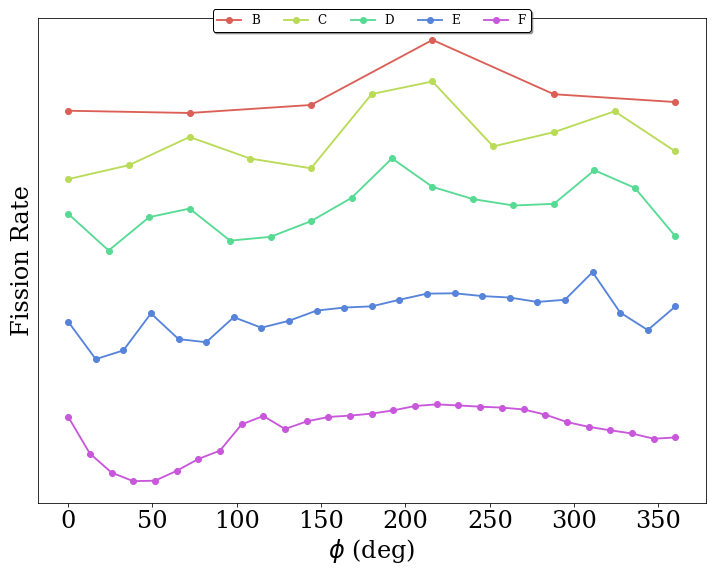
\includegraphics[height=5in]{tex/figures/totals_azi.png}
\caption[Whole Core Azimuthal Fission Rate Density]{The fission rate density for each element in the core as a function of core position.}
\label{fig:totals_azi}
\end{figure}

By studying \FIG{fig:totals_azi}, one can again see the effect the NEBP has on the F ring's fission rates.
This depression is seen when sweeping past the NEBP from around 12$^{\circ}$-75$^{\circ}$.
Other peaks and vally's seen in the figure are likely the cause of control rod, central thimble, and source placement.


% ------------------------------------------------------------------------------
\section{Application of ADVANTG}

% ------------------------------------------------------------------------------
\section{Tally Results}
